%
% Titelpagina
%

\maketitle


%
% Copyright
%

\null
\vfill

Copyright © 2011 Tim Besard

\vspace{1cm}

\begin{wrapfigure}{l}{2.5cm}
\vspace{-16pt}
\centering
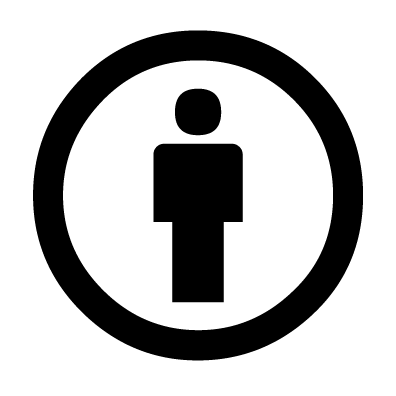
\includegraphics[width=2.5cm]{afbeeldingen/creative-commons-by}
\end{wrapfigure}

\noindent Dit werk valt onder de Belgische Creative Commons Attribution 2.0 licentie. Een kopie van deze licentie is te verkrijgen op de \makeurl{http://creativecommons.org/licenses/by/2.0/be/}{Creative Commons website}, of door een brief te sturen naar \texttt{Creative Commons, 171 Second Street, Suite 300, San Francisco, California, 94105, USA}.

\newpage


%
% Abstract
%

\chapter*{Abstract}
\addcontentsline{toc}{chapter}{Abstract}

\textit{Hier komt een abstract.}


%
% Voorwoord
%

\chapter*{Voorwoord}
\addcontentsline{toc}{chapter}{Voorwoord}

\textit{Hier komt het voorwoord.}


%
% Inhoudstafel
%

\setlength\cftpartnumwidth{2em}

\newpage
\tableofcontents

\newpage


%
% Lijst met afbeeldingen
%

\listoffigures


%
% Lijst met listings
%

\lstlistoflistings


%
% Lijst van afkortingen
%

\chapter*{Lijst van afkortingen}
\addcontentsline{toc}{chapter}{Lijst van afkortingen}

\begin{acronym}[WYSIWYG]	% langste afkorting

\acro{upnp}[UPnP]{Universal Plug and Play}
\acro{mdns}[mDNS]{Multicast DNS}
\acro{dns}[DNS]{Domain Name System}
\acro{ssdp}[SSDP]{Simple Service Discovery Protocol}
\acro{dcp}[DCP]{Device Control Protocol}
\acro{ssl}[SSL]{Secure Socket Layer}
\acro{rpc}[RPC]{Remote Procedure Call}
\acro{webdav}[WebDAV]{Web-based Distributed Authoring and Versioning}
\acro{http}[HTTP]{Hypertext Transport Protocol}
\acro{rmi}[RMI]{Remote Method Invocation}
\acro{corba}[CORBA]{Common Object Request Broker Architecture}
\acro{soap}[SOAP]{Simple Object Access Protocol}
\acro{wysiwyg}[WYSIWYG]{What You See Is What You Get}
\acro{html}[HTML]{Hypertext Markup Language}
\acro{rest}[REST]{Representational State Transfer}
\acro{jvm}[JVM]{Java Virtual Machine}
\acro{svn}[SVN]{Apache Subversion}
\acro{ram}[RAM]{Random Access Memory}
\acro{nas}[NAS]{Network Attached Storage}
\acro{gpu}[GPU]{Graphics Processing Unit}
\acro{dsp}[DSP]{Digital Signal Processor}
\acro{usb}[USB]{Universal Serial Bus}
\acro{hid}[HID]{Human Interface Device}
\acro{isp}[ISP]{In-System Programming}
\acro{hvsp}[HVSP]{High-Voltage Serial Programming}
\acro{uart}[UART]{Universal Asynchronous Receiver/Transmitter}
\acro{lufa}[LUFA]{Lightweight USB Framework for AVRs}
\acro{pll}[PLL]{Phase-Locked Loop}
\acro{dru}[DRU]{Design Rules}
\acro{pcb}[PCB]{Printed Circuit Board}
\acro{cpu}[CPU]{Central Processing Unit}
\acro{xml}[XML]{eXtensible Markup Language}
\acro{xsd}[XSD]{XML Schema Definition}
\acro{dhcp}[DHCP]{Dynamic Host Configuration Protocol}
\acro{ip}[IP]{Internet Protocol}
\acro{ajp}[AJP]{Apache JServ Protocol}
\acro{maven}[Maven]{Apache Maven}
\acro{pom}[POM]{Project Object Model}
\acro{jar}[JAR]{Java ARchive}
\acro{fpu}[FPU]{Floating-Point Unit}
\acro{api}[API]{Application Programming Interface}
\acro{eeprom}[EEPROM]{Electrically Erasable Programmable Read-Only Memory}
\acro{scpd}[SCPD]{Service Control Protocol Description}
\acro{ajax}[Ajax]{Asynchronous JavaScript and XML}
\acro{uuid}[UUID]{Universally Unique Identifier}
\acro{mac}[MAC]{Media Access Control}
\acro{moc}[MOC]{Meta-Object Compiler}
\acro{fsf}[FSF]{Free Software Foundation}
\acro{gpl}[GPL]{\acs{gnu} General Public License}
\acro{lgpl}[LGPL]{\acs{gnu} Lesser General Public License}
\acro{agpl}[AGPL]{\acs{gnu} Affero General Public License}
\acro{mpl}[MPL]{Mozilla Public License}
\acro{mit}[MIT]{Massachusetts Institute of Technology}
\acro{rhel}[RHEL]{Red Hat Enterprise Linux}
\acro{gnu}[GNU]{GNU's Not Unix!}
\acro{sl}[SL]{Scientific Linux}
\acro{wtfpl}[WTFPL]{Do What The Fuck You Want Public License}
\acro{ohl}[OHL]{Open Hardware License}
\acro{cc}[CC]{Creative Commons}
\acro{cc-by}[CC-BY]{\acl{cc} Attribution}
\acro{cc-sa}[CC-SA]{\acl{cc} ShareAlike}
\end{acronym}
